% Options for packages loaded elsewhere
\PassOptionsToPackage{unicode}{hyperref}
\PassOptionsToPackage{hyphens}{url}
\PassOptionsToPackage{dvipsnames,svgnames,x11names}{xcolor}
%
\documentclass[
  letterpaper,
  DIV=11,
  numbers=noendperiod,
  oneside]{scrartcl}

\usepackage{amsmath,amssymb}
\usepackage{iftex}
\ifPDFTeX
  \usepackage[T1]{fontenc}
  \usepackage[utf8]{inputenc}
  \usepackage{textcomp} % provide euro and other symbols
\else % if luatex or xetex
  \usepackage{unicode-math}
  \defaultfontfeatures{Scale=MatchLowercase}
  \defaultfontfeatures[\rmfamily]{Ligatures=TeX,Scale=1}
\fi
\usepackage{lmodern}
\ifPDFTeX\else  
    % xetex/luatex font selection
\fi
% Use upquote if available, for straight quotes in verbatim environments
\IfFileExists{upquote.sty}{\usepackage{upquote}}{}
\IfFileExists{microtype.sty}{% use microtype if available
  \usepackage[]{microtype}
  \UseMicrotypeSet[protrusion]{basicmath} % disable protrusion for tt fonts
}{}
\makeatletter
\@ifundefined{KOMAClassName}{% if non-KOMA class
  \IfFileExists{parskip.sty}{%
    \usepackage{parskip}
  }{% else
    \setlength{\parindent}{0pt}
    \setlength{\parskip}{6pt plus 2pt minus 1pt}}
}{% if KOMA class
  \KOMAoptions{parskip=half}}
\makeatother
\usepackage{xcolor}
\usepackage[left=1in,marginparwidth=2.0666666666667in,textwidth=4.1333333333333in,marginparsep=0.3in]{geometry}
\setlength{\emergencystretch}{3em} % prevent overfull lines
\setcounter{secnumdepth}{-\maxdimen} % remove section numbering
% Make \paragraph and \subparagraph free-standing
\ifx\paragraph\undefined\else
  \let\oldparagraph\paragraph
  \renewcommand{\paragraph}[1]{\oldparagraph{#1}\mbox{}}
\fi
\ifx\subparagraph\undefined\else
  \let\oldsubparagraph\subparagraph
  \renewcommand{\subparagraph}[1]{\oldsubparagraph{#1}\mbox{}}
\fi


\providecommand{\tightlist}{%
  \setlength{\itemsep}{0pt}\setlength{\parskip}{0pt}}\usepackage{longtable,booktabs,array}
\usepackage{calc} % for calculating minipage widths
% Correct order of tables after \paragraph or \subparagraph
\usepackage{etoolbox}
\makeatletter
\patchcmd\longtable{\par}{\if@noskipsec\mbox{}\fi\par}{}{}
\makeatother
% Allow footnotes in longtable head/foot
\IfFileExists{footnotehyper.sty}{\usepackage{footnotehyper}}{\usepackage{footnote}}
\makesavenoteenv{longtable}
\usepackage{graphicx}
\makeatletter
\def\maxwidth{\ifdim\Gin@nat@width>\linewidth\linewidth\else\Gin@nat@width\fi}
\def\maxheight{\ifdim\Gin@nat@height>\textheight\textheight\else\Gin@nat@height\fi}
\makeatother
% Scale images if necessary, so that they will not overflow the page
% margins by default, and it is still possible to overwrite the defaults
% using explicit options in \includegraphics[width, height, ...]{}
\setkeys{Gin}{width=\maxwidth,height=\maxheight,keepaspectratio}
% Set default figure placement to htbp
\makeatletter
\def\fps@figure{htbp}
\makeatother

<script src="../site_libs/htmlwidgets-1.6.2/htmlwidgets.js"></script>
<script src="../site_libs/viz-1.8.2/viz.js"></script>
<link href="../site_libs/DiagrammeR-styles-0.2/styles.css" rel="stylesheet" />
<script src="../site_libs/grViz-binding-1.0.11/grViz.js"></script>
\KOMAoption{captions}{tableheading}
\makeatletter
\makeatother
\makeatletter
\makeatother
\makeatletter
\@ifpackageloaded{caption}{}{\usepackage{caption}}
\AtBeginDocument{%
\ifdefined\contentsname
  \renewcommand*\contentsname{Table of contents}
\else
  \newcommand\contentsname{Table of contents}
\fi
\ifdefined\listfigurename
  \renewcommand*\listfigurename{List of Figures}
\else
  \newcommand\listfigurename{List of Figures}
\fi
\ifdefined\listtablename
  \renewcommand*\listtablename{List of Tables}
\else
  \newcommand\listtablename{List of Tables}
\fi
\ifdefined\figurename
  \renewcommand*\figurename{Figure}
\else
  \newcommand\figurename{Figure}
\fi
\ifdefined\tablename
  \renewcommand*\tablename{Table}
\else
  \newcommand\tablename{Table}
\fi
}
\@ifpackageloaded{float}{}{\usepackage{float}}
\floatstyle{ruled}
\@ifundefined{c@chapter}{\newfloat{codelisting}{h}{lop}}{\newfloat{codelisting}{h}{lop}[chapter]}
\floatname{codelisting}{Listing}
\newcommand*\listoflistings{\listof{codelisting}{List of Listings}}
\makeatother
\makeatletter
\@ifpackageloaded{caption}{}{\usepackage{caption}}
\@ifpackageloaded{subcaption}{}{\usepackage{subcaption}}
\makeatother
\makeatletter
\@ifpackageloaded{tcolorbox}{}{\usepackage[skins,breakable]{tcolorbox}}
\makeatother
\makeatletter
\@ifundefined{shadecolor}{\definecolor{shadecolor}{rgb}{.97, .97, .97}}
\makeatother
\makeatletter
\makeatother
\makeatletter
\@ifpackageloaded{sidenotes}{}{\usepackage{sidenotes}}
\@ifpackageloaded{marginnote}{}{\usepackage{marginnote}}
\makeatother
\makeatletter
\makeatother
\ifLuaTeX
  \usepackage{selnolig}  % disable illegal ligatures
\fi
\IfFileExists{bookmark.sty}{\usepackage{bookmark}}{\usepackage{hyperref}}
\IfFileExists{xurl.sty}{\usepackage{xurl}}{} % add URL line breaks if available
\urlstyle{same} % disable monospaced font for URLs
\hypersetup{
  pdftitle={Tree Equity Instructor Guide},
  colorlinks=true,
  linkcolor={blue},
  filecolor={Maroon},
  citecolor={Blue},
  urlcolor={Blue},
  pdfcreator={LaTeX via pandoc}}

\title{Tree Equity Instructor Guide}
\author{}
\date{}

\begin{document}
\maketitle
\ifdefined\Shaded\renewenvironment{Shaded}{\begin{tcolorbox}[frame hidden, boxrule=0pt, sharp corners, interior hidden, borderline west={3pt}{0pt}{shadecolor}, enhanced, breakable]}{\end{tcolorbox}}\fi

\hypertarget{what-is-data-science-and-why-urban-planning}{%
\subsection{What is Data Science and Why Urban
Planning}\label{what-is-data-science-and-why-urban-planning}}

\begin{itemize}
\tightlist
\item
  \textbf{Key Idea:} Data science is about extracting insight from data
  to inform action.
\item
  \textbf{Focus} on applications of data science that connect to
  students interests
\item
  Ask students to add their own example of data science they've seen and
  why they suspect it to be data science.
\end{itemize}

Emphasis on Data science and Urban Planning as a cycle that is
repetitive. There is always new data being collected and new solutions
to be found. This opens up possibilities for limitless data exploration
within the field which makes it an amazing introductory example of data
science for beginner students.

Urban Planning as reflection of Data science Cycle.

\hypertarget{tree-coverage-as-a-social-issue}{%
\subsection{Tree Coverage as a Social
Issue}\label{tree-coverage-as-a-social-issue}}

\begin{itemize}
\tightlist
\item
  \textbf{Remember} This concept might be difficult for students to
  grasp. ``How does the amount of trees in my neighborhood affect me?''
\item
  \textbf{Ask} Students, ``What does a tree do? What is its purpose''
  Answers might be ``Provides Shade'' or ``Creates Oxygen'' These are
  already good markers to highlight disparity but informing students of
  trees other functions and how their presence in a community or the
  lack thereof can make a large difference in the well-being of its
  members will help make their studies feel relevant and impactful.
\end{itemize}

\hypertarget{understanding-the-tree-equity-score}{%
\subsection{Understanding the Tree Equity
Score}\label{understanding-the-tree-equity-score}}

\href{https://www.treeequityscore.org/methodology}{Here} you can find
the methodology behind American Forests Tree Equity Research.

\begin{itemize}
\tightlist
\item
  The Tree Equity Score represents the \textbf{Need} for tree planting
  in an area. Need or Priority in a neighborhood is calculated by a
  number of factors that may highlight the potential for the area to be
  disproportionately affected by extreme heat, pollution and other
  environmental hazards which could be reduced with the benefits of
  trees.
\end{itemize}

\begin{marginfigure}

{\centering 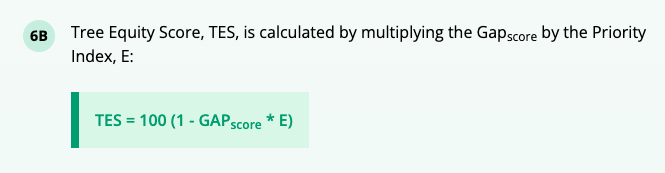
\includegraphics{TESCalc.png}

}

\end{marginfigure}

\hypertarget{foundational-learning}{%
\subsection{Foundational Learning}\label{foundational-learning}}

DS4HS places a priority on shifting the narrative on data scienc and its
accessibility. One of the main goals of this curriculum is to make
content as tangible as possible for those with experience in data or
statistical analysis. This section introduces key concepts in data
science and we want to make sure these concepts are grasped as
thoroughly as possible.

\begin{itemize}
\item
  \textbf{Observation vs.~Observational Unit:} Be explicit---each row is
  one observation, and the observational unit is the ``thing'' each row
  represents (e.g., a tree, a bus stop, a city block).In this example
  the ``GEOID'' represents one city block group
\item
  \textbf{Ask:} ``What is one row describing?'' Have students answer in
  plain language.
\item
  Variable Types: Clarify the difference between categorical and
  numerical variables. Use color/highlight in your slides or board to
  mark a few examples from the dataset. Students often confuse column
  headers for variable values. Reinforce that variables are columns,
  values are entries in rows.
\item
  If possible, have students follow along in R to observe the data set.
  This can help them get used to the variable names and what a typical
  value looks like for a given variable.
\end{itemize}

\hypertarget{mathlink-cubes}{%
\subsection{Mathlink Cubes}\label{mathlink-cubes}}

In every lesson, there is some for of interactive portion to help
students grasp the task of data wrangling through a physical simulation
of the practice.

This example comes from an article in the Journal of Statistics and Data
Science Learning.
\href{https://www.tandfonline.com/doi/citedby/10.1080/26939169.2025.2485234?scroll=top\&needAccess=true}{Using
Mathlink Cubes to Introduce Data Wrangling}\footnote{D'Agostino McGowan,
  L. (2025). Using Mathlink Cubes to Introduce Data Wrangling with
  Examples in R. Journal of Statistics and Data Science Education,
  1--10. https://doi.org/10.1080/26939169.2025.2485234} helps to
facilitate a tangible understanding of datasets and data manipulation.

This example can also be replicated with paper strips and squares
(though the creation of these materials may be tedious.)

\begin{itemize}
\tightlist
\item
  Hand out Mathlink Cubes to students in the form of ``a dataset''
  meaning cubes are arranged in columns by color. Dependending on the
  size of your data set(amount of rows), students will need that many
  blocks of a unique colored block for the mutate example.
\end{itemize}

\hypertarget{teaching-tidyverse-and-ggplot}{%
\subsection{Teaching tidyverse and
ggplot}\label{teaching-tidyverse-and-ggplot}}

\hypertarget{core-goals}{%
\subsubsection{Core Goals}\label{core-goals}}

\begin{itemize}
\item
  Students experience transforming a dataset using tidyverse data verbs
\item
  They start asking questions of the data: Who's impacted? Where? What
  relationships exist?
\item
  Students see visualization as a tool for insight, not just graphics.
\end{itemize}

\hypertarget{pedagogical-tips-and-emphases}{%
\subsubsection{Pedagogical Tips and
Emphases}\label{pedagogical-tips-and-emphases}}

\textbf{1. Emphasize the ``verbs'' as actions}

\begin{itemize}
\item
  Anchor each function to a mental model:

  \begin{itemize}
  \item
    \texttt{filter()} = ``cut out \textbf{rows} you don't need''
  \item
    \texttt{select()} = ``keep only the \textbf{columns} you care
    about''
  \item
    \texttt{mutate()} = ``make new columns using calucaltions with
    exsisting ones''
  \item
    \texttt{groupby()} = ``Sort data into baskets by value''
  \item
    \texttt{summarize()} = ``Pull out the big-picture''
  \end{itemize}
\end{itemize}

\textbf{2. Highlight data types when visualizing}

\begin{itemize}
\item
  Categorical → bar/column
\item
  Continuous → histogram, scatter
\item
  Time-based → line plot
\item
  Encourage asking: \emph{``What kind of variable is this? What would
  help me see patterns?''}
\end{itemize}

\textbf{3. Don't skip reading outputs}

\begin{itemize}
\item
  Stop after each code chunk and ask: \emph{``What changed? What does
  this output tell us?''}
\item
  It's easy for students to focus on syntax and miss what the data is
  really saying.
\end{itemize}

\textbf{4. Ask real-world connection questions}

\begin{itemize}
\item
  \emph{``What trend do you notice?'', ``What might explain that
  relationship?'', ``What other variable might influence both?''}
\item
  Encourage students to answer these questions in \textbf{normal} and
  \textbf{confortable} language rather than expecting a more refined
  ``data-sciency'' answer. This will help bridge the gap between their
  common sense and trained data analysis
\end{itemize}

\hypertarget{student-exploration-final-project}{%
\subsection{Student Exploration + Final
Project}\label{student-exploration-final-project}}

This capstone activity gives students the chance to apply everything
they've learned from the lesson. It should feel open-ended and
empowering, encouraging curiosity and creative problem-solving.

This is also the moment where data becomes personal and meaningful:
students choose their question, their variables, and their
visualization. The instructor's role shifts from direct teaching to
coaching, guiding students to sharpen questions, troubleshoot code, and
draw clear, grounded conclusions.

\hypertarget{group-work-guidance}{%
\subsubsection{Group Work Guidance}\label{group-work-guidance}}

Students should work in groups of 2--4, ideally with access to a shared
device

\textbf{Encourage them to:}

\begin{itemize}
\item
  Settle on a single state or comparison they find interesting.
\item
  Write out a clear, answerable question (this may take several
  revisions).
\end{itemize}

\textbf{Students will use R to generate at least one graph and one
statistical summary.}

Instructors or mentors should:

\begin{itemize}
\item
  Circulate and offer help with debugging.
\item
  Ask clarifying questions to refine vague research questions.
\item
  \emph{``What are you trying to compare? What variable would show
  that?''}
\end{itemize}

\hypertarget{managing-student-presentations}{%
\subsubsection{Managing Student
Presentations}\label{managing-student-presentations}}

Each group should give a short (\textasciitilde3--4 min) presentation
of: - Their question - What data they used - Their plot(s) and the
trends they suggest - A brief interpretation: \emph{``What does this
mean?''} and \emph{``Why does it matter?''}

\textbf{While students present:}

\begin{itemize}
\item
  Highlight clarity of visualizations, originality of questions, or
  insightful interpretations.
\item
  Celebrate one strong point from each group to model good data science
  communication:
\end{itemize}

``What I loved about this presentation was how clear the graph labels
were --- it helped us understand the pattern immediately.''



\end{document}
